% ---------------------------------------------------------------------
%  EE 545 Digital Signal Processing II -- Project Proposal
%  Gandhi Alexis Sinhue Contreras Torres
%
%  THIS .tex IS THE MASTER SOURCE.  Edit it directly.
%  Build:  julia build_pdf.jl      (runs pdflatex twice and tidies up)
%  Needs:  figures/architecture.png
%
%  Guideline checks: 3-5 pages, 11 pt, abstract <= 200 words,
%  background <= 1 page, project plan = largest section, >= 3 references.
% ---------------------------------------------------------------------
\documentclass[11pt,a4paper]{article}

\usepackage[a4paper,text={16.5cm,25.2cm},centering]{geometry}
\usepackage{lmodern}
\usepackage{amssymb,amsmath}
\usepackage{bm}
\usepackage{graphicx}
\makeatletter
\def\maxwidth{\ifdim\Gin@nat@width>\linewidth\linewidth\else\Gin@nat@width\fi}
\makeatother
\setkeys{Gin}{width=\maxwidth,keepaspectratio}
\usepackage{float}
\usepackage{tabularx}
% headings already carry their own numbers, so suppress LaTeX numbering
\setcounter{secnumdepth}{0}

\usepackage{microtype}
\usepackage{hyperref}
\setlength{\parindent}{0pt}
\setlength{\parskip}{1.2ex}

\hypersetup
       {   pdfauthor = { Gandhi Alexis Sinhue Contreras Torres },
           pdftitle={ Selective Event-Driven Encoding for Multimodal Robotic Sensing: Information, Rate and Reconstruction Tradeoffs },
           colorlinks=TRUE,
           linkcolor=black,
           citecolor=blue,
           urlcolor=blue
       }

\title{ Selective Event-Driven Encoding for Multimodal Robotic Sensing: Information, Rate and Reconstruction Tradeoffs }

\author{ Gandhi Alexis Sinhue Contreras Torres }

\date{ EE 545 Digital Signal Processing II -- Project Proposal }

% (Weave's listings/xcolor syntax-highlighting block removed: no code in this document.)

\begin{document}

\maketitle

\section{Abstract}

The usual question asked of event-driven sampling is whether it outperforms uniform
sampling. For a sensor-rich robot a more useful question is available, because some
signals are naturally change-driven while others carry dense information that a
threshold rule destroys. This project therefore asks: \textbf{which signals in a heterogeneous sensing
system deserve an event-driven representation, and which must stay continuously
sampled?} Using a Quanser QCar~2 as a sensor testbed, I will record a synchronized
multimodal dataset (wheel encoder, IMU, LiDAR, RGB-D depth, camera frames) and treat
four signal classes as separate cases: transition-dominated, mixed, sparse-geometric,
and dense-visual. For each I implement a level-crossing or change-detection encoder,
measure information retained against event rate, and fuse the surviving event streams
with the continuous streams into a single state estimate, evaluated against the Quanser
conventional full-rate fusion as reference. A self-recorded EEG experiment adds a fifth case,
testing whether the rule transfers to a broadband biological signal. Success is defined
by explicit numerical gates, not by showing an advantage: the deliverable is a
per-modality verdict from reconstruction error, event rate, task error and data volume,
including cases where event encoding proves wrong.

\section{Background}

Conventional DSP assumes a uniform sample clock, and the apparatus of this course rests
on it. Event-driven sampling drops that assumption: samples are emitted only when the
signal changes by a set amount, so sampling instants become signal dependent, the
Nyquist criterion no longer applies directly, and reconstruction error is set by the
threshold and the signal slew rate rather than by a rate. This is the course's
``bandpass and non-ideal sampling'' topic taken to its limit.

Existing work applies this idea unevenly. Hagenaars et al.~[1] estimate depth from event
streams alone and run it on-device, making the latency argument explicitly; Jing et
al.~[2] fuse event and frame streams asymmetrically, which is a multirate problem in
disguise; Wang et al.~[3] fuse radar with camera in a single stage. What these share is
that the \emph{choice} of which modality to represent as events is made in advance by
the hardware, never measured. Li et al.~[4] ask the complementary question for a real
2\,MB, 2.07\,GMAC/s DSP --- which published models actually fit --- and answer: none.
Accuracy is reported widely; the joint curve of accuracy against rate against precision
is reported rarely, and the per-modality question is not reported at all. Mitra~[5]
supplies the uniform-rate machinery (filter structures, multirate systems, coefficient
quantization) used here as the reference implementation.

This places the project in category~3 of the guidelines: implement alternative front
ends and compare their performance, including finite word-length effects, on signals
with different statistics.

\section{Project plan}

\begin{figure}[H]
\centering
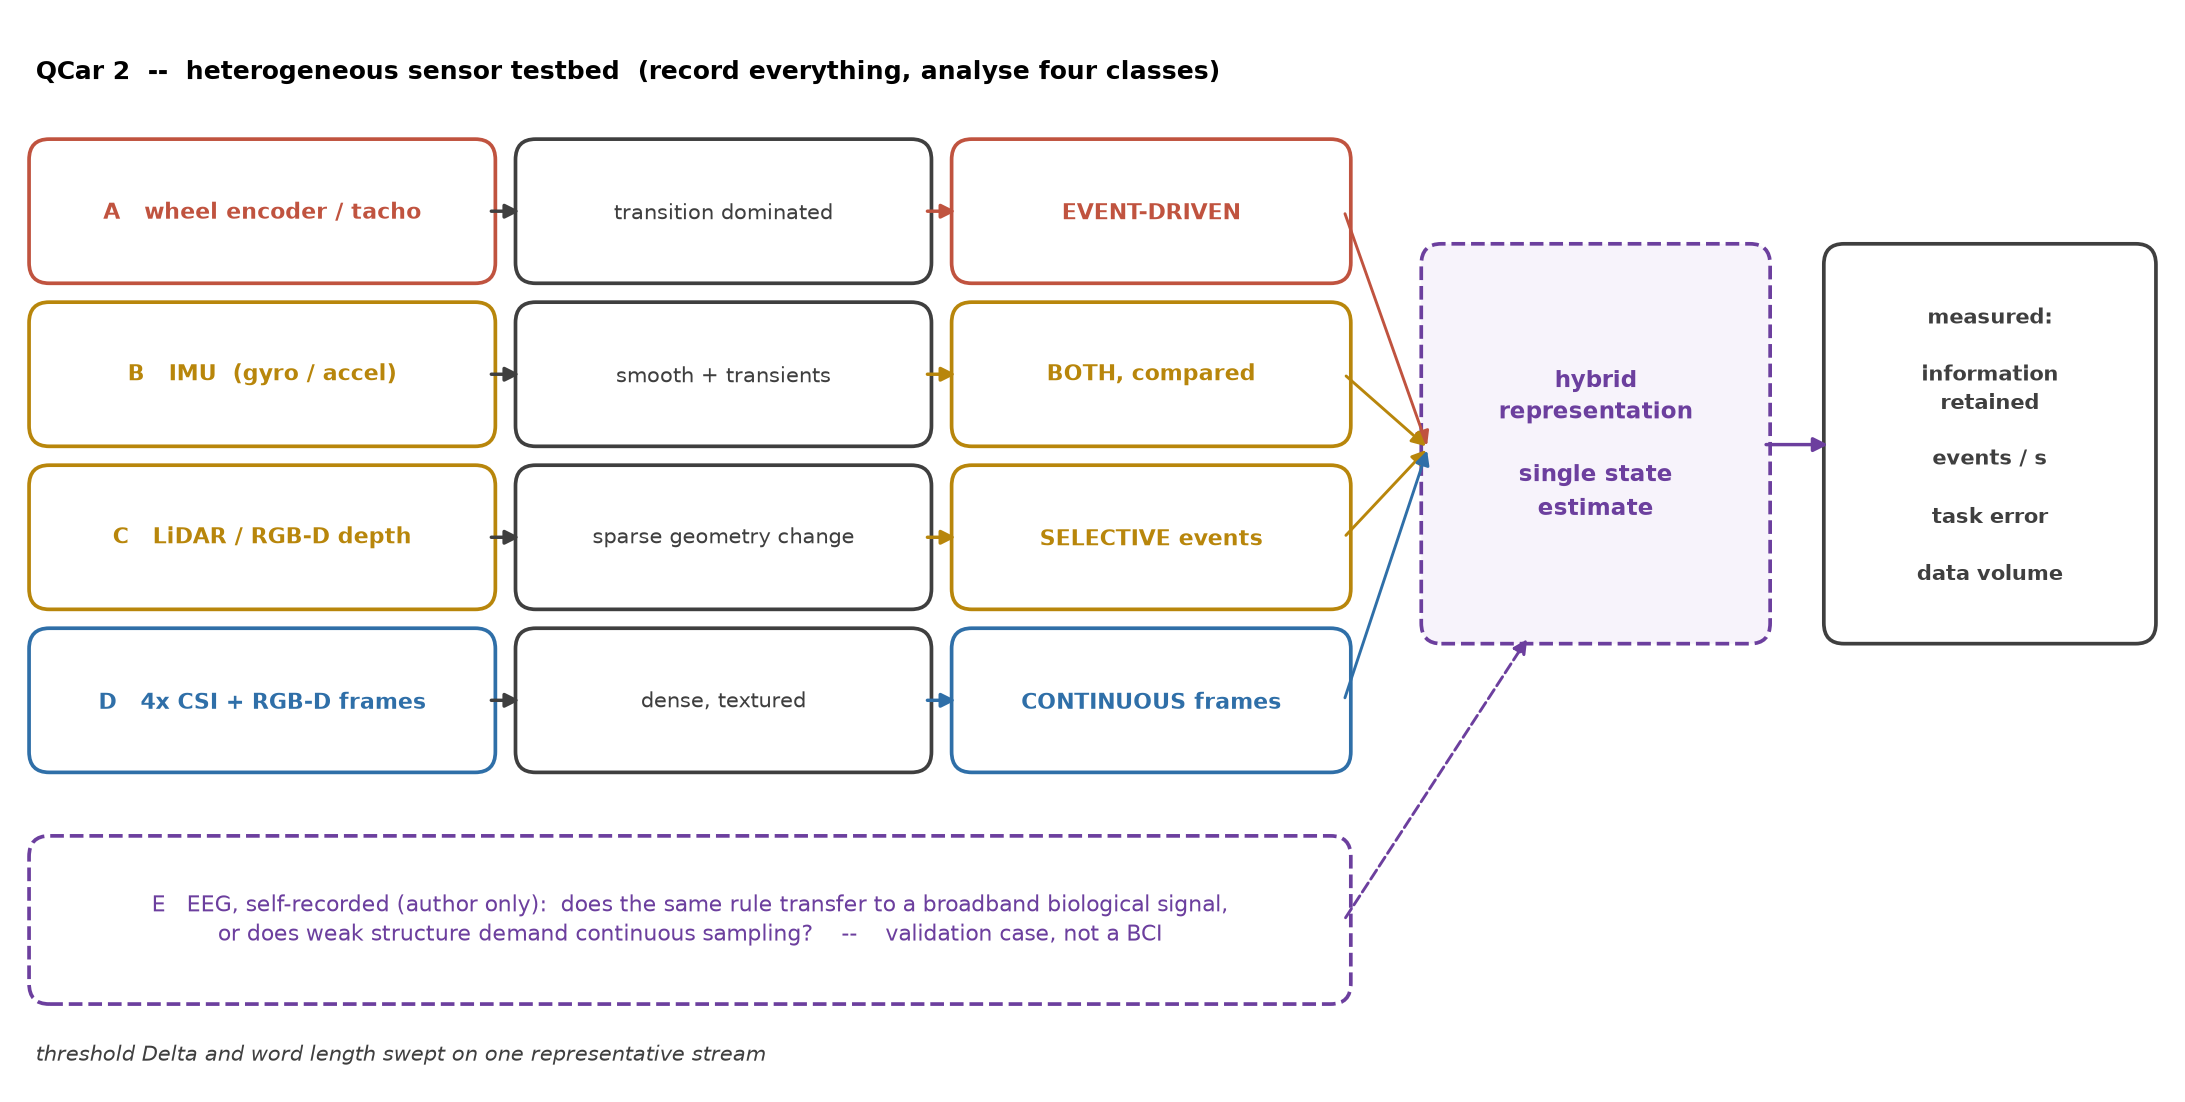
\includegraphics{figures/architecture.png}
\caption{Four robot signal classes, each with its own encoding verdict, fused into one
state estimate; EEG is a fifth validation case. The verdicts shown are hypotheses to be
tested, not assumptions.}
\end{figure}

\subsection{What already exists, and what is new for EE 545}

\textbf{Already in place before this course,} from my research and from the platform
vendor: QCar~2 and QDrone~2 hardware and access; the Quanser sensor APIs and the
conventional acquisition and sensor-fusion examples, which I already have running; and
my prior background in neuromorphic control and robotics. \emph{None of this is claimed
as work for this class.}

\textbf{New work performed specifically for EE 545:} (1) a synchronized multimodal
acquisition and the recorded dataset itself; (2) DSP characterization of each sensor
stream, including bandwidth and spectral content; (3) the event-encoding algorithms;
(4) the selective event/continuous architecture and its fusion stage; (5) the threshold
and rate sweeps; (6) reconstruction and feature-error analysis; (7) the rate-matched
conventional control; (8) the multimodal task comparison; (9) the EEG self-recording and
its representation experiment. Items 1--9 are the deliverable.

\subsection{Acquisition}

The QCar~2 carries four CSI cameras, an RGB-D camera, LiDAR, a 6-axis IMU and motor
encoders on a Jetson AGX Orin, which makes it a heterogeneous acquisition testbed rather
than a single-sensor platform. I will \emph{record} all available streams with synchronized acquisition
timestamps during scripted driving runs, then \emph{analyse} the four representative
classes below. \emph{Recording broadly but analysing selectively} is what keeps the scope
bounded. Processing is offline on the recorded dataset, which decouples the DSP study
from real-time execution timing and from lab availability. The QDrone~2 is a transfer
experiment only if time permits.

\subsection{The four robot cases}

For a scalar stream an event is emitted when $|x(t) - x_{\text{last}}| > \Delta$; for
inertial data I will additionally test a derivative rule $|dx/dt| > \gamma$; for frames
and depth, temporal change, $|I_k - I_{k-1}| > \Delta_I$ and $|D_k - D_{k-1}| > \Delta_D$.

\textbf{A. Wheel encoder / tachometer.} Already transition-dominated, so this is the
case most likely to favour events, and it supplies a natural event-driven reference
modality. The comparison is explicit: native encoder transition timestamps against a
conventionally sampled and reconstructed wheel velocity. Measure timestamp rate,
reconstructed velocity error, and data-rate reduction.

\textbf{B. IMU.} The ambiguous case, and therefore the interesting one. Compare uniform
sampling against level crossing and against derivative thresholding, separately for
steady motion and for aggressive steering and acceleration.

\textbf{C. LiDAR and RGB-D depth.} Test whether only significant geometric change needs
to be represented, using range sweeps and depth regions of interest.

\textbf{D. Camera frames.} I will \emph{not} synthesise a full event camera. I will
compare the regular frame stream against temporal-difference masks and
change-triggered region processing, and expect this case to argue \emph{against} event
encoding --- which is a result, not a failure. To keep the offline arithmetic tractable,
frame analysis operates on downsampled luminance and frame-difference matrices rather
than full-resolution colour.

\subsection{Hybrid fusion}

For the representative navigation streams, the surviving event and continuous
representations are combined in a hybrid state-estimation experiment, without
resampling everything to the fastest rate. Not every modality enters one estimator.
The reference is the Quanser conventional full-rate fusion output, and the task metric
is pose and trajectory RMSE against it. A
finite-word-length study (32-bit float versus 16- and 8-bit fixed point, including
coefficient quantization) is run on \emph{one} representative stream, for direct
alignment with the course topic without multiplying the experiment count.

\subsection{E. EEG self-recording}

Per Dr.~Creusere's guidance, EEG acquisition is restricted to \textbf{self-recording by
the author only}; no other participants are involved, and no multi-subject study is
attempted. The protocol is short and fixed: rest with eyes open, rest with eyes closed,
imagined left-hand movement, imagined right-hand movement, and actual hand open/close.
I will confirm any applicable institutional requirements before acquisition; publication
or any study involving other people is separate future work and is not claimed here.

No BCI classifier is required. The DSP question is whether change-driven representation
reduces EEG data volume while preserving the spectral features of interest, measured by
power spectral density, alpha/beta band power, reconstruction error and event rate.
Gate 3 applies here as it does to the robot cases: the level-crossing EEG stream is
compared against a uniformly decimated control at the same average rate, so that any
distortion in band power can be attributed either to the reduced rate or specifically
to non-uniform thresholding. The working hypothesis, carried over from the
smooth-versus-broadband contrast above, is that EEG will tolerate thresholding far
worse than the encoder or IMU streams because its information lives in low-amplitude
broadband structure.

\subsection{What I expect to learn}

Which modalities are naturally event-compatible, which are partially compatible, and
which require continuous representation --- and whether that ordering follows from
measurable signal statistics rather than from intuition.

\subsection{Explicitly out of scope}

No closed-loop or real-time control onto hardware; processing is offline on recorded
datasets. No synthesised full event camera. No multi-subject human-participant study:
EEG is limited to single-investigator self-recording for pilot validation. QDrone~2 is
an extension, not a committed deliverable.

\section{Metrics for Success}

Four headline axes are reported for every modality, produced by the same code path for
the continuous and the event condition so that differences are attributable to the
representation:

\begin{tabularx}{\linewidth}{@{}lX@{}}
\hline
Information retained & reconstruction SNR and NRMSE after hold reconstruction; for EEG, band-power error \\
Events per second & absolute event rate per stream \\
Data-rate reduction & $CR_{\text{data}} = (\text{continuous bytes/s}) / (\text{event bytes/s})$, comparable across all modalities \\
Task degradation & pose/trajectory RMSE against the Quanser conventional full-rate reference \\
Computation / data volume & MAC per second of signal, and bytes per second \\
\hline
\end{tabularx}

Headline plots: RMSE versus event rate; feature error versus event rate; bandwidth
versus threshold; task error versus data reduction.

\subsection{Test rubrics: what counts as success}

These are the pass/fail criteria. The project is judged against them, not against
whether event encoding wins.

\begin{enumerate}
\item \textbf{Encoder round trip.} As $\Delta$ decreases toward zero, NRMSE must
decrease and the event rate must approach the original sampling rate. Fails if that
trend does not hold. This verifies the encoder before any result is believed.
\item \textbf{Synchronization.} Cross-correlation of a common excitation across streams
must align them to within one sample of the slowest stream. Fails if timestamps cannot
be aligned, in which case fusion results are not reported.
\item \textbf{Rate-matched control.} Any claimed event advantage must survive comparison
against the uniform pipeline decimated to the same average rate. An advantage that
disappears here is a data-volume effect, not a representation effect, and is reported as
such.
\item \textbf{Fusion reference.} The hybrid state estimate must track the Quanser
conventional reference with RMSE no worse than a stated tolerance at the lowest
threshold tested; otherwise the fusion stage, not the encoding, is at fault.
\item \textbf{Per-modality verdict.} Each of cases A--E must end with a defensible
one-line verdict (event / hybrid / continuous) supported by its own measured curve.
Producing five supported verdicts is the definition of a complete project.
\end{enumerate}

\textbf{Success} means gates 1--5 pass and the four axes are reported for all five
cases, \emph{whatever the verdicts turn out to be}. A finding that only the encoder
benefits, and that cameras and EEG should stay continuous, fully answers the research
question. \textbf{Failure} means the gates cannot be passed, which would mean the
measurements are not trustworthy.

\subsection{Schedule}

\begin{tabularx}{\linewidth}{@{}lX@{}}
\hline
Oct 6 & QCar~2 synchronized multimodal recording; verify gate 2; set up EEG self-recording \\
Oct 13 & Level-crossing and change encoders; reconstruction SNR versus $\Delta$; gate 1 \\
Oct 20 & Cases A and B (encoder, IMU); rate-matched control; gate 3 \\
Oct 27 & Cases C and D (LiDAR/depth, frames) \\
Nov 3 & Hybrid fusion; pose/trajectory RMSE against the Quanser reference; gate 4 \\
Nov 10 & EEG self-recording and spectral/representation analysis (case E) \\
Nov 17 & Finite word-length study on one representative stream; headline plots \\
Nov 24 & Buffer; draft report \\
Dec 1 & Final report and presentation \\
\hline
\end{tabularx}

\section{References}

\begin{enumerate}
\item J. J. Hagenaars, Y. Wu, F. Paredes-Vall\'es, S. Stroobants, G. C. H. E. de Croon, ``On-device self-supervised learning of low-latency monocular depth from only events,'' \emph{CVPR}, 2025.
\item L. Jing, D. Shi, Y. Cao, Y. Wang, J. Zhang, Y. Cui, M. Wang, ``AIMDepth: Asymmetric image-event Mamba for monocular depth estimation,'' \emph{CVPR}, 2026.
\item Y. Wang et al., ``TacoDepth: Towards efficient radar-camera depth estimation with one-stage fusion,'' \emph{CVPR}, 2025.
\item J. Li, L. Liu, K. Malsky, G. Yi, ``Real-time music source separation on a low-power audio DSP,'' Analog Devices, Inc.
\item S. K. Mitra, \emph{Digital Signal Processing: A Computer-Based Approach}, 4th ed., McGraw-Hill.
\item Quanser Inc., ``QCar 2 product specifications,'' \url{https://www.quanser.com/products/qcar-2/}.
\item S. Zare, S. I. Beaber, Y. Sun, ``NeuroFlex: Feasibility of EEG-based motor imagery control of a soft glove for hand rehabilitation,'' \emph{Sensors}, vol. 25, no. 3, p. 610, 2025.
\end{enumerate}

\end{document}
